\chapter{Experimental Results}
\label{ch:results}

This chapter reports the evaluation of seven detectors across four tiers on the
benchmark. It states the research questions and the experimental setup, then
presents the headline results, the per-CWE detection on clean code, the
adversarial robustness results, and a per-tier analysis of the LLMs, the trained
model, and the whole-project detectors. It closes with the effect of the label
filter and a summary.

%----------------------------------------------------------

\section{Research Questions and Setup}

The evaluation answers three questions. \textbf{RQ1:} how accurately do the
detectors classify the seven sink-shaped CWE classes on clean code? \textbf{RQ2:}
how does each detector's accuracy change under a semantics-preserving mutator,
and which mutator exposes the most brittleness? \textbf{RQ3:} does the diff-based
label filter change the picture a detector evaluation paints? The purpose is to
show what the benchmark measures, not to rank detectors.

The held-out test set is 129 samples (67 positives across the seven classes, 62
safe negatives). Every detector is scored one-versus-rest per CWE under five
bounded measures: macro-F1, detection MCC on the binary vulnerable-versus-safe
collapse, Severity-Weighted Recall (SWR) on the 27 CVSS-scored positives,
Hierarchical CWE Macro-Accuracy (HCMA), and weighted Cohen's $\kappa$. The
robustness drop is clean macro-F1 minus mutated macro-F1 over the 67 positives.
The seven detectors are Bandit and Semgrep (pattern-matching SAST), Snyk Code
and CodeQL (whole-project dataflow), Claude Sonnet 4.6, GPT-4o, and DeepSeek R1
(LLMs), and a fine-tuned GraphCodeBERT.

\section{Results Analysis}

\subsection{Headline Results}

Table~\ref{tab:headline} reports the seven detectors. No single tool leads on
every measure. DeepSeek R1 takes the top macro-F1 (0.596); Sonnet 4.6 leads SWR
(0.903) and HCMA (0.805); the trained GraphCodeBERT leads detection MCC
($+0.556$); and Bandit edges weighted $\kappa$ ($+0.567$). The two LLMs Sonnet
and GPT-4o sit below the SAST and learned tiers on MCC because they over-flag
hard negatives as CWE-22 and CWE-918. Snyk Code is an outlier on every detection
metric (macro-F1 0.063), which is read as a property of the single-function
format rather than a ranking.

\begin{table}[htb]
\caption{Detector results on the 129-sample clean test set. Macro-F1 is
one-versus-rest across seven CWEs; MCC is on the binary vulnerable/safe collapse;
SWR is severity-weighted recall on the 27 CVSS-scored positives; HCMA is
hierarchical accuracy; $\kappa_w$ is weighted Cohen's $\kappa$; Comp.\ is
macro-F1 on the composed mutator; $\Delta$F1$^\star$ is the worst-case
single-mutator drop (positives only).}
\label{tab:headline}
\centering
\resizebox{\textwidth}{!}{%
\begin{tabular}{lrrrrrrr}
\toprule
\textbf{Detector} & \textbf{macro-F1} & \textbf{MCC} & \textbf{SWR} & \textbf{HCMA} & $\boldsymbol{\kappa_w}$ & \textbf{Comp.} & $\boldsymbol{\Delta}$\textbf{F1}$^{\star}$ \\
\midrule
Bandit               & 0.510 & $+0.478$ & 0.745 & 0.564 & $\mathbf{+0.567}$ & 0.589 & $+0.187$ \\
Semgrep              & 0.315 & $+0.157$ & 0.634 & 0.353 & $+0.227$ & 0.375 & $+0.132$ \\
Snyk Code            & 0.063 & $-0.235$ & 0.143 & 0.069 & $-0.097$ & 0.088 & $+0.036$ \\
Claude Sonnet 4.6    & 0.585 & $+0.117$ & $\mathbf{0.903}$ & $\mathbf{0.805}$ & $+0.396$ & 0.867 & $0.000$ \\
GPT-4o               & 0.356 & $+0.047$ & 0.420 & 0.419 & $+0.295$ & 0.565 & $+0.026$ \\
DeepSeek R1          & $\mathbf{0.596}$ & $+0.410$ & 0.691 & 0.646 & $+0.539$ & 0.567 & $+0.068$ \\
GraphCodeBERT (ours) & 0.524 & $\mathbf{+0.556}$ & 0.870 & 0.547 & $+0.548$ & 0.603 & $0.000$ \\
\bottomrule
\end{tabular}}
\end{table}

The hierarchical and agreement columns sharpen the comparison between Bandit and
the trained detector. On macro-F1 Bandit (0.510) trails GraphCodeBERT (0.524) by
0.014, but on HCMA the gap inverts and Bandit (0.564) edges ahead (0.547).
Bandit's errors are dominated by close-sibling mistakes inside the injection
subtree, which Wu-Palmer credits as partial matches but macro-F1 scores as flat
misses. Weighted $\kappa$ agrees: Bandit ($+0.567$) and GraphCodeBERT ($+0.548$)
are within 0.019 of each other. Bandit and the trained detector are therefore
comparable on clean code under any partial-credit metric.

\subsection{Detection on Clean Code (RQ1)}

Among the SAST and learned tiers, detectors diverge most on SQL injection: Bandit
reaches F1 0.80 on CWE-89 by lexically matching inline SQL, GraphCodeBERT 0.63,
and Semgrep only 0.06 because its taint-shape rules require a
framework-recognizable source-to-sink shape absent from the fragmentary samples.
CWE-22 scores zero for all three (no usable rule, too few training samples), and
CWE-918 separates the tiers: both SAST tools score zero while GraphCodeBERT
recovers F1 0.57. Table~\ref{tab:clean-percwe} gives the per-class breakdown.

\begin{table}[htb]
\caption{Per-CWE F1 on the clean test set ($n$ = positive test samples). GCB is
the trained GraphCodeBERT detector.}
\label{tab:clean-percwe}
\centering
\begin{tabular}{lrrrr}
\toprule
\textbf{CWE} & $n$ & \textbf{Bandit} & \textbf{Semgrep} & \textbf{GCB} \\
\midrule
CWE-22  Path Traversal       &  3 & 0.00 & 0.00 & 0.00 \\
CWE-78  OS Command Injection &  4 & 0.38 & 0.29 & 0.40 \\
CWE-79  Cross-site Scripting &  7 & 0.60 & 0.33 & 0.67 \\
CWE-89  SQL Injection        & 32 & 0.80 & 0.06 & 0.63 \\
CWE-94  Code Injection       &  6 & 0.92 & 0.80 & 0.57 \\
CWE-502 Insecure Deserial.   & 12 & 0.83 & 0.73 & 0.83 \\
CWE-918 SSRF                 &  3 & 0.00 & 0.00 & 0.57 \\
\midrule
Macro-F1 (positives $+$ safe) &   & 0.51 & 0.32 & 0.52 \\
\bottomrule
\end{tabular}
\end{table}

\subsection{Adversarial Robustness (RQ2)}

The mutator families split the tiers apart, shown in
Table~\ref{tab:robustness}. The two pattern-matching SAST tools show a robustness
cliff on the sink-targeted family: Bandit drops 0.187 macro-F1 under attribute
obfuscation and 0.143 under builtins indirection; Semgrep drops 0.109 and 0.132.
The cliff replicates across two mutators attacking disjoint sink classes, so it
is a property of lexical sink-matching rather than a single trick. The trained
GraphCodeBERT detector is invariant to every mutator ($|\Delta\textrm{F1}|\le
0.036$), as are all three LLMs. All detectors are invariant to the four
sink-preserving mutators and to the dataflow mutator, the latter because none of
the current detectors performs dataflow analysis, so M7 remains a coverage slot
for future dataflow-aware tools.

\begin{table}[htb]
\caption{Macro-F1 by variant over the 67 positives. DC/SS/VR/WE:
sink-preserving; SAO/SVG: sink-targeted; TTD: dataflow; Comp: composed.}
\label{tab:robustness}
\centering
\resizebox{\textwidth}{!}{%
\begin{tabular}{lrrrrrrrrr}
\toprule
\textbf{Tool} & \textbf{Clean} & DC & SS & VR & WE & SAO & SVG & TTD & Comp \\
\midrule
Bandit        & 0.59 & 0.59 & 0.59 & 0.59 & 0.59 & 0.40 & 0.45 & 0.59 & 0.58 \\
Semgrep       & 0.38 & 0.38 & 0.38 & 0.38 & 0.38 & 0.28 & 0.25 & 0.37 & 0.38 \\
GraphCodeBERT & 0.57 & 0.59 & 0.60 & 0.60 & 0.61 & 0.60 & 0.57 & 0.60 & 0.60 \\
\bottomrule
\end{tabular}}
\end{table}

Table~\ref{tab:drop} reports the drops grouped by family in both macro-F1 and
severity-weighted recall. The SAST cliff is visible on the sink-targeted columns
(Bandit loses up to 0.347 SWR) and absent on the learned detector.

\begin{table}[htb]
\caption{Robustness drop (clean $-$ mutator) by family. Sink-preserve is the
mean of the four sink-preserving mutators; SAO, SVG, and TTD are individual.
$\Delta$SWR is the drop in severity-weighted recall.}
\label{tab:drop}
\centering
\resizebox{\textwidth}{!}{%
\begin{tabular}{lrrrrrrrr}
\toprule
& \multicolumn{2}{c}{Sink-preserve} & \multicolumn{2}{c}{SAO} & \multicolumn{2}{c}{SVG} & \multicolumn{2}{c}{TTD} \\
\cmidrule(lr){2-3}\cmidrule(lr){4-5}\cmidrule(lr){6-7}\cmidrule(lr){8-9}
\textbf{Tool} & $\Delta$F1 & $\Delta$SWR & $\Delta$F1 & $\Delta$SWR & $\Delta$F1 & $\Delta$SWR & $\Delta$F1 & $\Delta$SWR \\
\midrule
Bandit        & $+$.001 & .000  & $+$.187 & $+$.347 & $+$.143 & $+$.246 & .000  & .000 \\
Semgrep       & $+$.005 & .000  & $+$.109 & $+$.196 & $+$.132 & $+$.246 & $+$.018 & $-$.029 \\
GraphCodeBERT & $-$.036 & $+$.009 & $-$.035 & $+$.034 & .000  & .000  & $-$.030 & .000 \\
\bottomrule
\end{tabular}}
\end{table}

\subsection{Per-CWE Validation Progression}

Figure~\ref{fig:fp-progression} shows the per-CWE audit false-positive rate
across the three validation rounds. The diff filter collapses the
co-changed-file classes (CWE-502, CWE-94) to 0\%, while the residual noise
concentrates on CWE-89 and CWE-79, where \texttt{vudenc} samples are retained
without a paired fix to diff against.

\begin{figure}[htb]
\centering
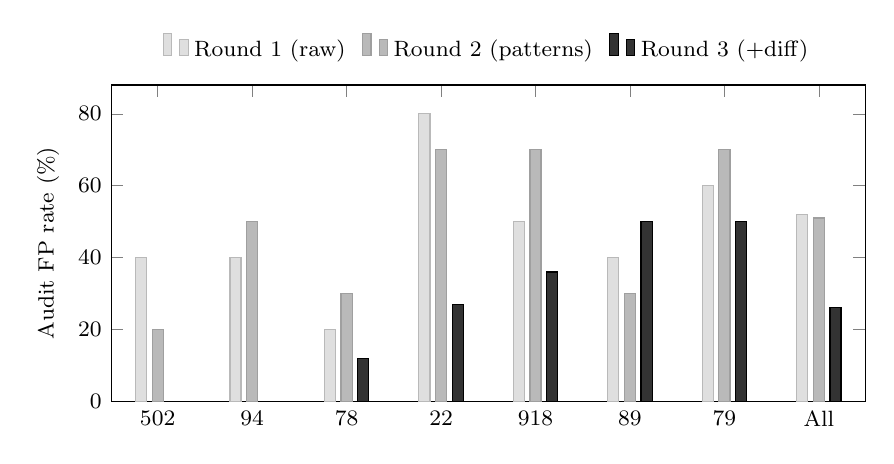
\begin{tikzpicture}
\begin{axis}[
  width=0.92\textwidth, height=5.6cm,
  ybar, bar width=4.0pt,
  ymin=0, ymax=88,
  ylabel={Audit FP rate (\%)},
  ylabel style={font=\footnotesize},
  symbolic x coords={502,94,78,22,918,89,79,All},
  xtick=data,
  x tick label style={font=\footnotesize},
  ytick={0,20,40,60,80},
  y tick label style={font=\footnotesize},
  legend style={at={(0.5,1.04)}, anchor=south, legend columns=3,
    font=\footnotesize, draw=none,
    /tikz/every even column/.append style={column sep=4pt}},
  enlarge x limits=0.07,
  tick align=inside,
]
\addplot+[fill=gray!25, draw=gray!55] coordinates {(502,40)(94,40)(78,20)(22,80)(918,50)(89,40)(79,60)(All,52)};
\addplot+[fill=gray!55, draw=gray!75] coordinates {(502,20)(94,50)(78,30)(22,70)(918,70)(89,30)(79,70)(All,51)};
\addplot+[fill=black!80, draw=black]   coordinates {(502,0)(94,0)(78,12)(22,27)(918,36)(89,50)(79,50)(All,26)};
\legend{Round 1 (raw), Round 2 (patterns), Round 3 ($+$diff)}
\end{axis}
\end{tikzpicture}
\caption{Per-CWE audit false-positive rate across the three validation rounds
(x-axis labels are CWE numbers; \emph{All} is the aggregate). The diff filter
collapses the co-changed-file classes to 0\% while the residual concentrates on
CWE-89 and CWE-79.}
\label{fig:fp-progression}
\end{figure}

\section{Detailed Analysis}

\subsection{LLM Detectors}

The three LLMs differ. DeepSeek R1 posts the highest macro-F1 in the
table (0.596) and the highest CWE-89 F1 of any detector (0.935); its MCC
($+0.410$) is the best of the three LLMs. Sonnet 4.6 ranks just below on macro-F1
(0.585) and takes the SWR (0.903) and HCMA (0.805) leads of the whole table, but
its MCC ($+0.117$) is low because it over-flags hard negatives as CWE-22 (15
false positives) and CWE-918 (17). GPT-4o is the weakest LLM (macro-F1 0.356,
MCC $+0.047$ near chance): it reaches F1 0.915 on CWE-89 but scores zero on
CWE-94 and over-applies CWE-22 and CWE-918 to safe code, a miscalibration rather
than a uniform weakness. All three are invariant to the mutators, which confirms
that the sink-token cliff is a property of lexical SAST, not of the mutator
suite.

\subsection{Trained-Model Detector}

The fine-tuned GraphCodeBERT reaches macro-F1 0.524 and the table-leading
detection MCC ($+0.556$), which reflects a lower false-positive rate on hard
negatives than either SAST tool or any LLM. It is invariant to every mutator,
including the sink-targeted family that breaks the SAST tools, because it draws
on semantic features beyond the sink identifier. This is a defensible small-data
existence proof: 610 samples is small for a 126.6M-parameter model, so the
result shows that a benchmark-tuned learned detector can compete with mature
baselines on Python sink-shaped CWEs, not that it is state of the art.

\subsection{Whole-Project Dataflow Detectors}

Snyk Code is built for whole-application analysis but is scored here on
single-function extracts; it flags 1 of 32 CWE-89 positives and produces many
false positives on the safe class, because the framework source-to-sink lineage
it tracks is absent from the extracts. CodeQL returned zero findings for the same
reason: its source model requires application entry points the extracts do not
contain. This is a property of the benchmark format, not the tools, and both
detector implementations are kept in the released harness for a future
application-level benchmark.

\subsection{Effect of the Label Filter (RQ3)}

The numbers above use the diff-filtered labels (26\% audited false positive). Run
against unfiltered labels, every tool's apparent precision falls by construction,
because a tool that correctly declines a mislabeled sample is charged a false
negative. The filter therefore does not flatter the tools; it removes samples on
which a correct detector and a wrong label disagree.

\section{Summary}

Across seven detectors in four tiers, no single tool leads on every measure, and
the sink-token mutator family is the axis that separates pattern-matching SAST,
which drops up to 0.187 macro-F1, from a learned detector invariant to every
mutator. The validation progression in Figure~\ref{fig:fp-progression} shows
where label noise was removed, and the label-filter analysis shows that the
filter tightens rather than inflates the scores. Chapter~\ref{ch:conclusion}
draws conclusions and states limitations and future work.
